\documentclass[mathserif]{beamer}
%\documentclass[mathserif,handout]{beamer}
%\documentclass[dvips]{beamer}
\definecolor{Beige}{rgb}{0.96,0.96,0.86}
\definecolor{Yellow}{rgb}{1.,0.84,0.8}
\definecolor{Gold}{rgb}{1.,0.84,0.}
\definecolor{RedA}{hsb}{0.9,0.3,0.7}
\definecolor{RedB}{hsb}{0.9,0.3,1}
\definecolor{LightGray}{gray}{0.85}
\definecolor{Blue}{rgb}{0.,0.,1.}
\definecolor{Pink}{rgb}{0.9,0.75,0.8}
\definecolor{DarkGreen}{rgb}{1.0,1.0,1.0}
\definecolor{DarkBlue}{rgb}{0.,0.5,1.0}
%\definecolor{Pink}{rgb}{1.,0.75,0.8}
\definecolor{LightCyan}{rgb}{0.88,1.,1.}
%\definecolor{LightYellow}{rgb}{0.95,1.0,0.8}
\definecolor{red1}{rgb}{0.95,0.,0.}
%\definecolor{mycol1}{rgb}{0.9,0.2,0.9}
%\definecolor{mycol1}{rgb}{0.5,0.8,0.4}
\definecolor{mycol1}{rgb}{0.5,0.6,0.8}
\definecolor{mycol2}{rgb}{0.6,0.8,0.6}
\definecolor{LightYellow}{rgb}{0.95,1.0,0.8}

\mode<presentation>
{
%\usepackage{beamerthemeCambridgeUS, fancybox}
\usepackage{fancybox}
\usepackage{graphicx}
\usepackage{subfigure}
\usepackage[english]{babel}
\usepackage{multirow}
\usepackage{verbatim}
\usepackage{verbatim,epsfig,graphics,amssymb,amsmath,subfigure}
\usepackage{helvet}
\usepackage{graphicx}
\usepackage{wrapfig}
\setbeamercovered{transparent}
}
%\usepackage[T1]{fontenc}
%\usepackage[adobe-utopia]{mathdesign}
%\usepackage{fouriernc}
\usepackage[bitstream-charter]{mathdesign}
\usepackage[T1]{fontenc}



\usefonttheme{serif}

\usetheme{Boadilla} 

\setbeamertemplate{navigation symbols}{}
\setbeamersize{text margin left=3mm, text margin right=3mm}
\newcommand{\B}[1]{\boldsymbol{#1}}
\usepackage[all]{xy}
\usepackage[utf8]{inputenc}
%\usepackage{pdfpages}
\renewcommand{\footnotesize}{\scriptsize}

\title[Seed-grant proposal]
{Multimodal classification of birds\\
\small{Seed-grant proposal}}

%\author[Paddy]{R. Padmanabhan (Paddy)}
\author[ADP]{Arnav Bhavsar\\
		Dileep A. D.\\
		Padmanabhan Rajan
}

\institute[IIT Mandi] {
Multimedia Analytics and Systems Lab\\
School of Computing and Electrical Engineering\\
%Indian Institute of Technology Mandi \\

\includegraphics[width=4cm,height=2cm]{figures/mas_logo.pdf}

\includegraphics[width=3cm,height=2cm]{figures/iitmandi-logo.pdf}
}
%\date[November 11th, 2009]
{}

%%%%%%%%%%%%%%%%%%%%%%%%%%%%%%%%%%%%%%%%%%%%%%%%%%%%%%%%%%%%%%%%%%%%%%%%%%%%%%%%%%%%%%%%%%%%%
\begin{document}
\normalfont

%%%%%%%%%%%%%%%%%%%%%%%%%%%%%%%%%%%%%%%%%%%%%%%%%%%%%%%%%%%%%%%%%%%%%%%%%%%%%%%%
\begin{frame}
        \titlepage
\end{frame}

%\logo{
\includegraphics[height=0.8cm]{figures/iitmandi-logo.pdf}\vspace{220pt}}
\logo{
\includegraphics[height=0.8cm]{figures/mas_logo.pdf}\vspace{220pt}}

\begin{frame}
\frametitle{Overview}
\begin{wrapfigure}{r}{0.5\textwidth}
\centering
%  \begin{center}
    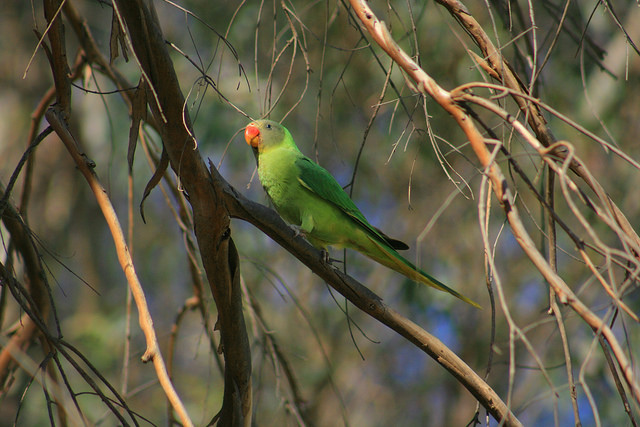
\includegraphics[width=0.48\textwidth]{figures/parakeet.jpg}
%  \end{center}
  \caption{\small{Slaty-headed parakeet. Pic by PPJ.}}
\end{wrapfigure}
The objective\\
The acoustics\\
The image/video\\
The machine learning\\
The budget and other details\\
\end{frame}

\begin{frame}
\frametitle{The objective}
\begin{itemize}
\item<2-> Develop algorithms for automatic analysis of avian biodiversity
\item<3-> Combine information from acoustic and visual data streams
\item<4-> Sensors: microphones, cameras
\item<5-> Apply signal processing and machine-learning techniques to collected
data
\item<6-> Tasks: Species identification, species detection
\end{itemize}
\end{frame}

\begin{frame}
\frametitle{The motivation}
\begin{itemize}
\item<2-> Birds provide crucial ecosystem services: pollination, seed dispersal,
insectivory
\item<3-> Avian diversity: good indicator of ecosystem health in a local area
\item<4-> Automatic and semi-automatic sensing devices can be utilized
\item<5-> Large volume of data captured by these devices
\item<6-> Algorithms to analyze this data would be useful to ecologists
\item<7-> Our campus location in the lower Himalayas: sensitive ecosystem
\item<8-> Proposed system can be used for long-term ecological monitoring
\end{itemize}
\end{frame}

\begin{frame}
\frametitle{The challenges}
\begin{itemize}
\item<2-> Challenges at various levels
\item<3-> Acoustics:
	\begin{itemize}
	\item<4-> Complex acoustic environment where recordings are made
	\item<5-> Overlapping vocalizations, intra-species call variability
	\item<6-> Background sounds (other animals, human-made sounds, river etc.)
	\end{itemize}
\item<8-> Image/video: 
	\begin{itemize}
	\item<9-> Complex visual environment, visual background clutter
	\item<10-> Overlapping inter-class visual appearances, local variations  
	\item<11-> Intra-class variations: robustness to changes in pose, motion, light conditions.
	\end{itemize}
% \item<12-> Fusion of modalities
% 	\begin{itemize}
% 	\item<13-> Curating of feature vectors and subsystem decisions 
% 	\item<14-> Complementary representations from different modalities
% 	\item<15-> Correlating sound and videos
% 	\end{itemize}
\item<12-> Machine-learning:
	\begin{itemize}
	\item<13-> Fixed-length representations and varying-length representations
	\item<14-> Dynamic kernels for bird data from different modalities
	\item<15-> Fusion of modalities
	\begin{itemize}
	    \item<16-> Combining the representations from acoustic and image/video modes
	    \item<17-> Combining the decisions from the classifiers for the representations from acoustic and image/video modes
	\end{itemize}
	\item<18-> Bird indexing and retrieval
	\end{itemize}
\end{itemize}
\end{frame}


\begin{frame}
\frametitle{The acoustics (cont'd)}
\begin{itemize}
\item<2-> Processing of human speech: techniques can be adapted for birdcalls
\item<3-> Production mechanisms are different, but have similarities (eg. formant
structure)
\item<4-> Existing techniques include:
\begin{itemize}
	\item spectral representations \footnote{
	H. Tyagi et. al., ``Automatic identification of birdcalls using spectral 
	ensemble average voice prints'', Proc. EUSIPCO, 2006},
	\item Mel frequency cepstra \footnote{M. Graciarena et. al., 
	``Acoustic front-end optimization for bird species recognition'', 
	Proc. ICASSP, 2010}, 
	\item hidden Markov models \footnote{M. Graciarena et.al., 
	``Bird species recognition combining acoustic and sequence modeling'', 
	Proc. ICASSP, 2011}, 
	\item sparse representations \footnote{L. N. Tan et. al. 
	``Evaluation of a sparse representation-based classifier for bird phrase 
	classification", Proc. Interspeech, 2012}
\end{itemize}
\end{itemize}
\end{frame}


\begin{frame}
\frametitle{The acoustics (cont'd)}
\begin{itemize}
\item<2-> Research focus: \textcolor{blue}{subspace representations} 
\item<3-> A recording can be represented as a fixed-length vector $\mathbf{x}$ 
\item<4-> Can be used for various applications, for eg. removing background
sounds before classification:
\begin{itemize}
	\item<5-> Project $\mathbf{x}$ into a subspace of background sounds, and remove this
	component from $\mathbf{x}$
\end{itemize}
\item <6-> Fixed-length representations: utilized in kernel functions for
support vector machines (SVMs)
\item <7-> Varying-length representations: conventional approach
\end{itemize}
\end{frame}


\begin{frame}
\frametitle{The visual: research areas}
\begin{itemize}
\item<2-> Fine-grained classification (of birds): relatively recent ($\geq$ 2010)
\item<3-> Learning visual guidance: inverse problem to classification \\$\Rightarrow$ Given the classes, find the discriminative features
\item<4-> Detection, segmentation and tracking of birds: \\Adapting general object detection, segmentation and tracking methods in computer vision
\item<5-> Sound source localization in videos: \\Adapting existing work in non-specific domains: \\Challenges for birds: less visual motion, background sounds
\end{itemize}
\end{frame}

\begin{frame}
\footnotesize
\frametitle{The visual: existing work}
\begin{itemize}
	\item<2-> Fine-grained classification 
	\begin{itemize}
	\footnotesize
	\item P. Welinder et. al., ``Caltech-UCSD Birds 200'',  CNS-TR-2010-001. 2010.
	\item T. Berg and P. Belhumeur, ``POOF: Part-based one-vs-one features for fine-Grained categorization, face verification, and attribute estimation'', CVPR 2013.
	\item L. Xie et. al., ``Hierarchical part matching for fine-grained visual categorization'', ICCV 2013.
	\item B. Yao et. al., ``A codebook-free and annotation-free approach for fine-grained image categorization'', CVPR 2012.	
	\end{itemize}	
	\begin{figure}
	\begin{tabular}{c c c}
	\only<3->{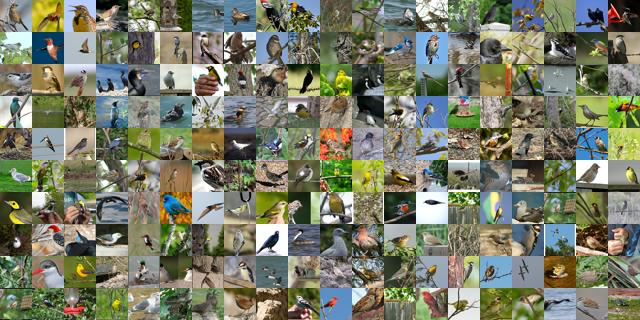
\includegraphics[height=2cm]{figures/collage.png}&
	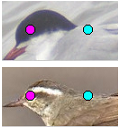
\includegraphics[height=1cm]{figures/bird_points.png}&
	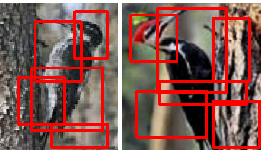
\includegraphics[height=1cm]{figures/bird_templates.png}}
	\end{tabular}
	\end{figure}
	\item<4-> Visual guidance: T. Berg and P. Belhumeur, ``How do you tell a
	blackbird from a crow?'', ICCV 2013.
	\item<5-> Detection: D. Song and Y. Xu, ``A monocular vision-based low false
	negative filter for assisting the search for rare bird species using a
	probable observation data set-based EKF method'', IEEE Trans. 
	Image Processing, 2010.	
\begin{figure}
\begin{tabular}{c c}
\only<6->{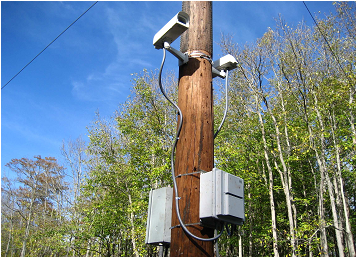
\includegraphics[height=1.5cm]{figures/cam.png}&
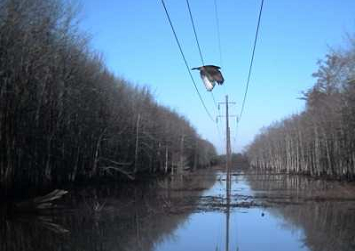
\includegraphics[height=1.5cm]{figures/detect.png}}
\end{tabular}
\end{figure}
\end{itemize}
\end{frame}

\begin{frame}
\frametitle{The visual: some possible directions}
\begin{itemize}
\item<2-> Features: 
\begin{itemize}
\item Patch-based features: review, feature selection, part identification
\item Body-part features: local appearance and geometric relationships
\item Feature learning: deep neural networks
\end{itemize}
\item<3-> Frameworks:
\begin{itemize}
\item Sparse representation: feature selection, classification
\item Markov Random Fields: segmentation, pose estimation
\item Hierarchical classification and visual guidance
\end{itemize}
\item<4-> Systems:
\begin{itemize}
\item Dataset collection
\item Audio-video systems for monitoring
\item On-board algorithms: detection, tracking
\item Online bird classification portal (image and sound)
\end{itemize}
\end{itemize}
\end{frame}



\begin{frame}
\frametitle{Example on-field system components}
\vspace{-1cm}
%Automatic analysis of birdcalls: fairly active research area\\
\vspace{0.3cm}
%\pause
\begin{itemize}
\item Data acquisition (audio): rugged, field-deployable recorders \\
e.g.~Song Meter SM3 recorder from Wildlife Acoustics Inc, USA \\
\item Data acquisition (video): Network cameras \\
e.g.~Panasonic WV-SP302\\
\item Processing: Raspberry Pi, Beagle Bone 
\end{itemize}
\begin{figure}
	\begin{tabular}{c c c}
	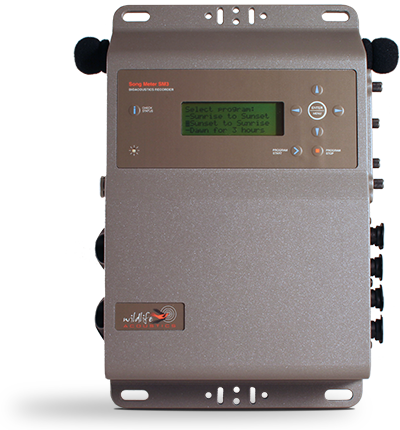
\includegraphics[height=3cm]{figures/songMeter.png}&
	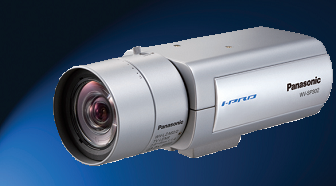
\includegraphics[height=2cm]{figures/pan_cam.png}&
	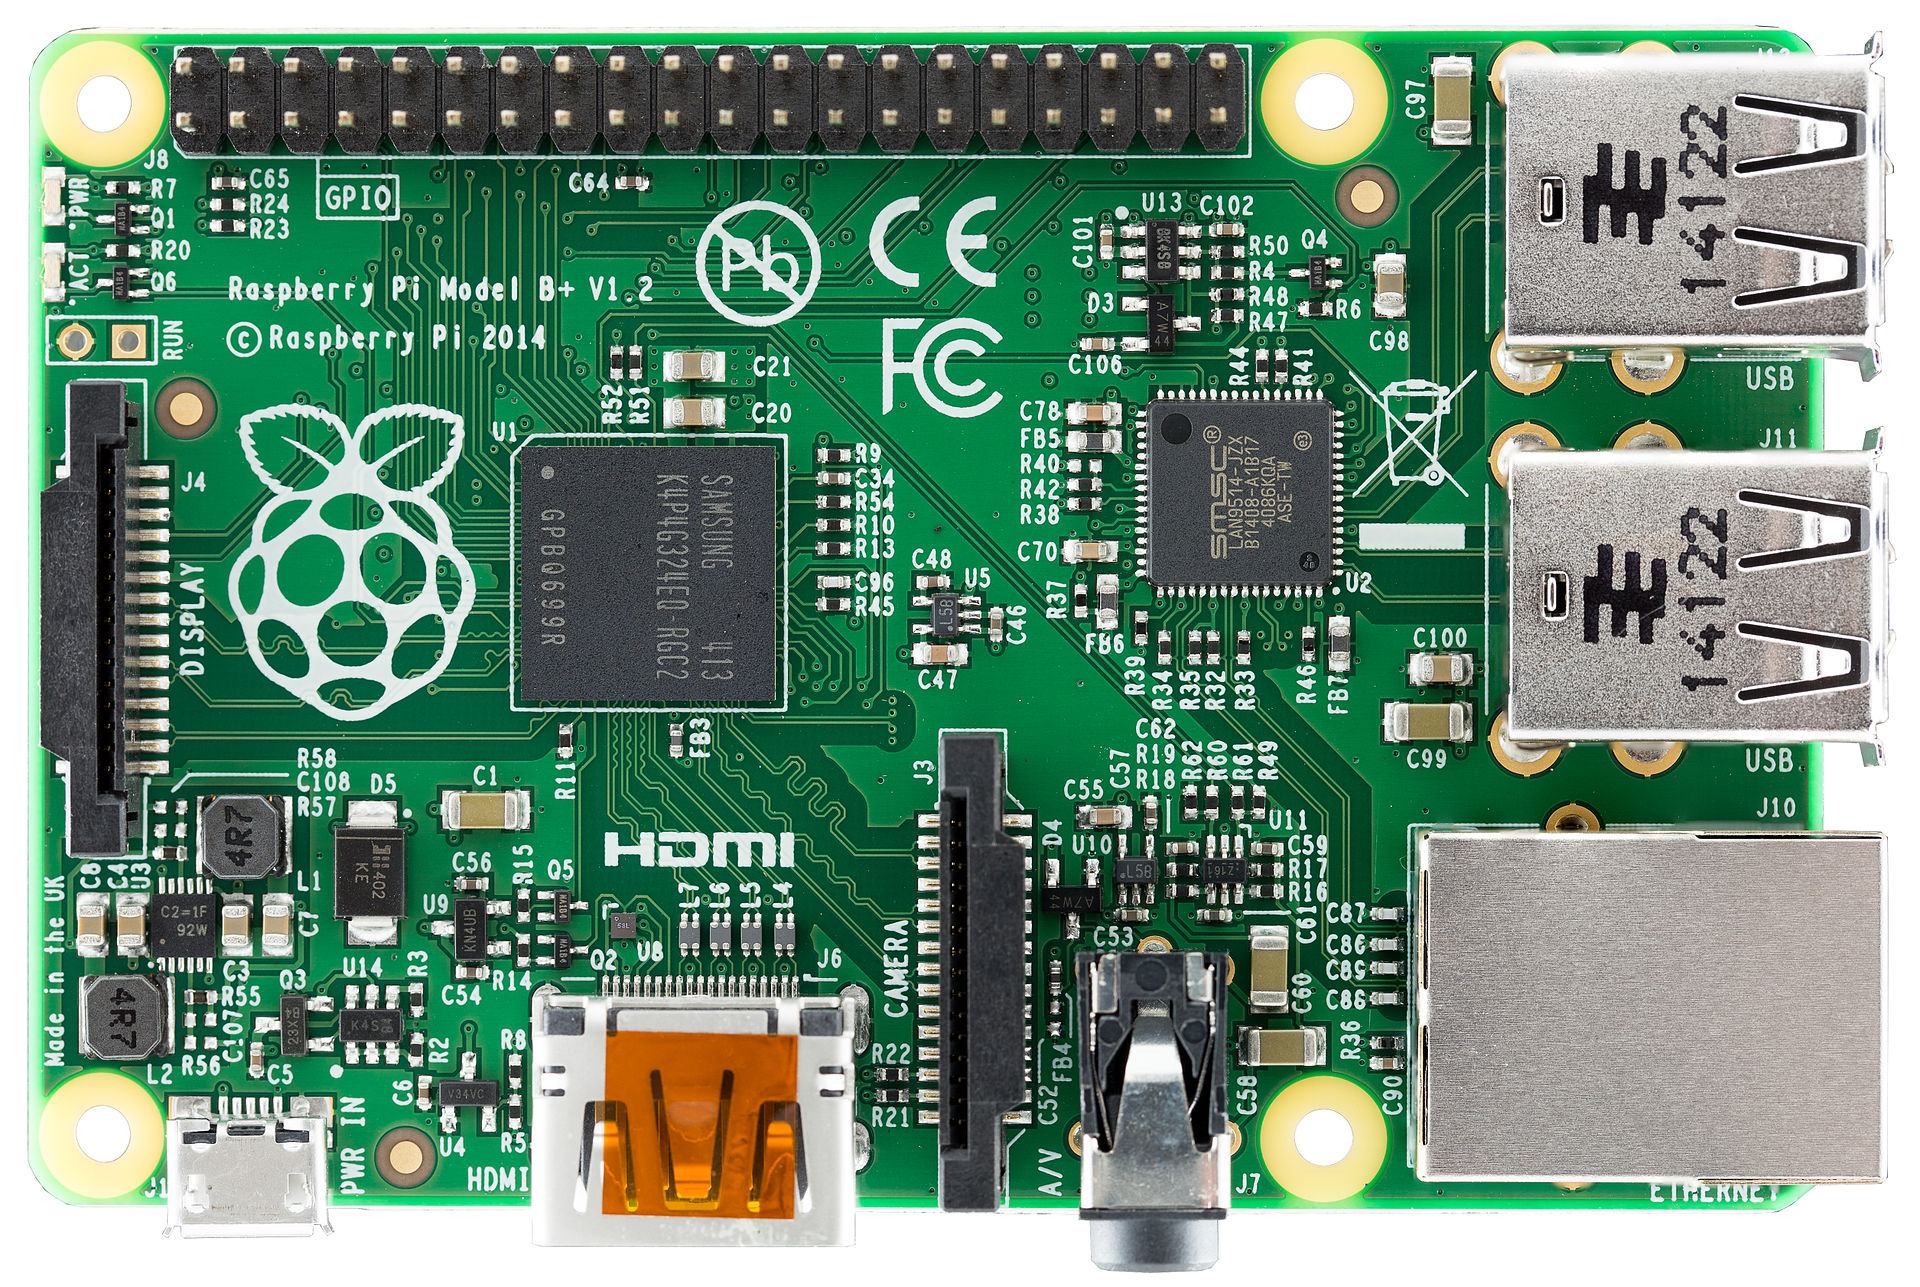
\includegraphics[height=2cm]{figures/rasp.jpg}
	\end{tabular}
	\end{figure}
\end{frame}


\begin{frame}
\frametitle{The machine learning: tasks}
\begin{itemize}
\item<2-> Birdcall identification 
\item<3-> Bird classification from images and videos
\item<4-> Birdcall indexing and retrieval
\item<5-> Bird image and video indexing and retrieval
\item<6-> Combining different modalities for classification, indexing and retrieval tasks
\end{itemize}
\end{frame}

\begin{frame}
\frametitle{The machine learning: bird classification}
\begin{itemize}
\item<2-> Classification of birds using SVMs from birdcalls and bird images \& videos
\item<3-> The representations for birdcall are either fixed-length
representation or varying-length representation
\item<4-> Varying-length representation are either sets of local feature vectors or sequences of local feature vectors
\item<5-> Dynamic kernel based SVMs for varying-length representation
\end{itemize}
\end{frame}

\begin{frame}
\frametitle{The machine learning: bird classification (cont'd)}
\begin{itemize}
\item<2-> Some of the dynamic kernels are:
\begin{itemize}
	\item GMM-based intermediate matching kernel \footnote{
	A. D. Dileep et. al., ``GMM-Based intermediate matching kernel for classification of varying length patterns of long duration speech using SVMs'', in IEEE TNNLS, Aug. 2014},
	\item HMM-based intermediate matching kernel \footnote{A. D. Dileep et. al., ``HMM-based intermediate matching kernel for classification of sequential patterns of speech using SVMs'', in IEEE TASLP, Dec. 2013}, 
	\item Histogram intersection kernel \footnote{J. C. van Gemert et. al., ``Visual word ambiguity'', in IEEE TPAMI, July 2010} 
	\item Spatial pyramid match kernel \footnote{S. Lazebnik et. al., ``Beyond bags of features: Spatial pyramid matching for recognizing natural scene categories'', in Proceedings of CVPR, June 2006} \end{itemize}
\end{itemize}
\end{frame}

\begin{frame}
\frametitle{The machine learning: bird indexing and retrieval}
\begin{itemize}
\item<2-> Matching and retrieval of birds using birdcalls and bird images \& videos
\begin{itemize}
      \item Query-by-example (QBE) based retrieval\footnote{
	A. Marakakis et. al., ``Probabilistic relevance feedback approach for content-based image retrieval based on Gaussian mixture models'', in IET Image Processing, Feb. 2009}
      \item Query-by-semantics (QBS) based retrieval\footnote{
	G. Carneiro et. al., ``Supervised learning of semantic classes for image annotation and retrieval'', in IEEE TPAMI, March 2007}
      \item Query-by-semantic example (QBSE) based retrieval\footnote{
	N. Rasiwasia et. al., ``Bridging the gap: Query by semantic example'' in IEEE Transactions on Multimedia, Aug. 2009}
\end{itemize}
\item<3-> Matching and retrieval of birds using kernel methods\footnote{
	T. Veena, ``Image classification, matching and annotation using kernel methods for content based image retrieval for scene images'', Ph.D. Thesis, Dept. of CSE, IIT Madras, June 2014}   
\end{itemize}
\end{frame}

\begin{frame}
\frametitle{The machine learning: multimodal classification and retrieval}
\begin{itemize}
\item<2-> Classification and retrieval of birds by combining the cues from birdcalls and bird images \& videos
\begin{itemize}
      \item Early fusion: Combining the acoustic, image and video features
      \item Late fusion: Combining the decisions from the different classifiers built for birdcalls, bird images and bird videos
 \end{itemize}
\item<3-> Feature selection and combining using multiple kernel learning
\end{itemize}
\end{frame}

\begin{frame}
\frametitle{Future plans: further funding}
\begin{itemize}
\item \textbf{Proposal to SERB:} 
	\begin{itemize}
	\item \textit{Automatic analysis of avian acoustics} 
	\item In collaboration with IIT Madras, NCBS and CDAC 
	\item PI from IIT Mandi: Padmanabhan Rajan
	\item Value: Rs 50 lakhs
	\item \textbf{Ready for submission}
	\end{itemize}

\item \textbf{Proposal planned:} \\Camera and acoustic sensor networks for a local area (IIT Mandi)
\end{itemize}
\end{frame}

\begin{frame}
\frametitle{}
\begin{center}
\Large{Thank you for your attention.}
\end{center}
\end{frame}


\begin{frame}
\frametitle{Budget and other details}

\begin{table}[th]
\centering
\caption{Projected expenses in lakhs INR.}
\begin{tabular}{|l|c|c|c|c|}
\hline
Items & Year 1 & Year 2 & Year 3 & Total\\
\hline
High-end computers (2) & 3.0 & 3.0 & 0 & 6.0\\
Imaging and audio equipment & 5.0 & 3.0 & 0 & 8.0 \\
Desktop computers (6) & 5.0 & 0 & 0 & 5.0  \\
Contingency & 0.5 & 0.5 & 1.0 & 2.0 \\
Travel & 0.5 & 0.5 & 1.0 & 2.0\\
\hline
Overall & 15.0 & 8.0 & 2.0 & \textbf{23.0} \\
\hline
\end{tabular}
\label{tab:funding}
\end{table}
\end{frame}


\begin{frame}
\frametitle{Equipment budget}

\begin{table}[th]
\centering
\caption{Equipment budget in thousands INR.}
\begin{tabular}{|l|c|c|c|}
\hline
Item & Unit cost & Qty. & Total\\
\hline
Bioacoustic recorder & 50 & 6 & 300 \\
Network camera & 30 & 5 & 150  \\
Recorder accessories & 15 & 8 & 120 \\
DSLR camera and lens & 100 & 1 & 100\\
Consumables & 50 & 1 & 50\\
Processing hardware & 8 & 5 & 40 \\
Network access points & 3 & 5 & 15\\
\hline
Total &  & & \textbf{775} \\
\hline
\end{tabular}
\label{tab:equipFunding}
\end{table}
\end{frame}





\end{document}


